\begin{figure}[H]
    \centering
    \begin{minipage}[t]{0.48\textwidth}
    \centering

    \begin{tikzpicture}[scale=0.8]
        \fill[gray] (1, 0) rectangle (2, 1);
        \fill[gray] (2, 0) rectangle (3, 1);
        \fill[gray] (3, 0) rectangle (4, 1);
        \fill[gray] (2, 1) rectangle (3, 2);
        \fill[gray] (0, 2) rectangle (1, 3);
        \node at (3.5, 2.5){\color{blue}\faIcon{home}};
        \fill[gray] (4, 2) rectangle (5, 3);
        \node at (1.5, 3.5){\color{blue}\faIcon{user}};
        \fill[gray] (2, 3) rectangle (3, 4);
        \fill[gray] (0, 4) rectangle (1, 5);
        \fill[gray] (4, 4) rectangle (5, 5);
        \draw[black] grid (5, 5);
    \end{tikzpicture}

    \caption{\centering Wybierz pole (1,3) jako następnie rozpatywany węzeł.}
    \label{fig:dfs_solve_steps_start}
    \end{minipage}\hfill
    \begin{minipage}[t]{0.48\textwidth}

    \centering

    \begin{tikzpicture}[scale=0.8]
        \fill[gray] (1, 0) rectangle (2, 1);
        \fill[gray] (2, 0) rectangle (3, 1);
        \fill[gray] (3, 0) rectangle (4, 1);
        \fill[gray] (2, 1) rectangle (3, 2);
        \fill[gray] (0, 2) rectangle (1, 3);
        \node at (3.5, 2.5){\color{blue}\faIcon{home}};
        \fill[gray] (4, 2) rectangle (5, 3);
        \node at (1.5, 3.5){\color{blue}\faIcon{user}};
        \fill[gray] (2, 3) rectangle (3, 4);
        \fill[gray] (0, 4) rectangle (1, 5);
        \fill[gray] (4, 4) rectangle (5, 5);
        \draw[black] grid (5, 5);
    \end{tikzpicture}

    \caption{\centering Oznacz pole (1,3) jako kandydata na ścieżkę.}
    \end{minipage}
\end{figure}

\begin{figure}[H]
\centering
\begin{minipage}[t]{0.48\textwidth}

  \centering

  \begin{tikzpicture}[scale=0.8]
    \fill[gray] (1, 0) rectangle (2, 1);
    \fill[gray] (2, 0) rectangle (3, 1);
    \fill[gray] (3, 0) rectangle (4, 1);
    \fill[gray] (2, 1) rectangle (3, 2);
    \fill[gray] (0, 2) rectangle (1, 3);
    \node at (1.5, 2.5){\color{purple}\faIcon{hourglass}};
    \node at (3.5, 2.5){\color{blue}\faIcon{home}};
    \fill[gray] (4, 2) rectangle (5, 3);
    \node at (1.5, 3.5){\color{blue}\faIcon{user}};
    \fill[gray] (2, 3) rectangle (3, 4);
    \fill[gray] (0, 4) rectangle (1, 5);
    \fill[gray] (4, 4) rectangle (5, 5);
    \draw[black] grid (5, 5);
  \end{tikzpicture}

  \caption{\centering Wybierz pole (1,2) jako następnie rozpatywany węzeł.}
\end{minipage}\hfill
\begin{minipage}[t]{0.48\textwidth}

  \centering

  \begin{tikzpicture}[scale=0.8]
    \fill[gray] (1, 0) rectangle (2, 1);
    \fill[gray] (2, 0) rectangle (3, 1);
    \fill[gray] (3, 0) rectangle (4, 1);
    \fill[gray] (2, 1) rectangle (3, 2);
    \fill[gray] (0, 2) rectangle (1, 3);
    \node at (1.5, 2.5){\color{orange}\faIcon{arrows-alt}};
    \node at (3.5, 2.5){\color{blue}\faIcon{home}};
    \fill[gray] (4, 2) rectangle (5, 3);
    \node at (1.5, 3.5){\color{blue}\faIcon{user}};
    \fill[gray] (2, 3) rectangle (3, 4);
    \fill[gray] (0, 4) rectangle (1, 5);
    \fill[gray] (4, 4) rectangle (5, 5);
    \draw[black] grid (5, 5);
  \end{tikzpicture}

  \caption{\centering Oznacz pole (1,2) jako kandydata na ścieżkę.}
\end{minipage}
\end{figure}

\begin{figure}[H]
\centering
\begin{minipage}[t]{0.48\textwidth}

  \centering

  \begin{tikzpicture}[scale=0.8]
    \fill[gray] (1, 0) rectangle (2, 1);
    \fill[gray] (2, 0) rectangle (3, 1);
    \fill[gray] (3, 0) rectangle (4, 1);
    \node at (1.5, 1.5){\color{purple}\faIcon{hourglass}};
    \fill[gray] (2, 1) rectangle (3, 2);
    \fill[gray] (0, 2) rectangle (1, 3);
    \node at (1.5, 2.5){\color{orange}\faIcon{arrows-alt}};
    \node at (3.5, 2.5){\color{blue}\faIcon{home}};
    \fill[gray] (4, 2) rectangle (5, 3);
    \node at (1.5, 3.5){\color{blue}\faIcon{user}};
    \fill[gray] (2, 3) rectangle (3, 4);
    \fill[gray] (0, 4) rectangle (1, 5);
    \fill[gray] (4, 4) rectangle (5, 5);
    \draw[black] grid (5, 5);
  \end{tikzpicture}

  \caption{\centering Wybierz pole (1,1) jako następnie rozpatywany węzeł.}
\end{minipage}\hfill
\begin{minipage}[t]{0.48\textwidth}

  \centering

  \begin{tikzpicture}[scale=0.8]
    \fill[gray] (1, 0) rectangle (2, 1);
    \fill[gray] (2, 0) rectangle (3, 1);
    \fill[gray] (3, 0) rectangle (4, 1);
    \node at (1.5, 1.5){\color{orange}\faIcon{arrows-alt}};
    \fill[gray] (2, 1) rectangle (3, 2);
    \fill[gray] (0, 2) rectangle (1, 3);
    \node at (1.5, 2.5){\color{orange}\faIcon{arrows-alt}};
    \node at (3.5, 2.5){\color{blue}\faIcon{home}};
    \fill[gray] (4, 2) rectangle (5, 3);
    \node at (1.5, 3.5){\color{blue}\faIcon{user}};
    \fill[gray] (2, 3) rectangle (3, 4);
    \fill[gray] (0, 4) rectangle (1, 5);
    \fill[gray] (4, 4) rectangle (5, 5);
    \draw[black] grid (5, 5);
  \end{tikzpicture}

  \caption{\centering Oznacz pole (1,1) jako kandydata na ścieżkę.}
\end{minipage}
\end{figure}

\begin{figure}[H]
\centering
\begin{minipage}[t]{0.48\textwidth}

  \centering

  \begin{tikzpicture}[scale=0.8]
    \fill[gray] (1, 0) rectangle (2, 1);
    \fill[gray] (2, 0) rectangle (3, 1);
    \fill[gray] (3, 0) rectangle (4, 1);
    \node at (0.5, 1.5){\color{purple}\faIcon{hourglass}};
    \node at (1.5, 1.5){\color{orange}\faIcon{arrows-alt}};
    \fill[gray] (2, 1) rectangle (3, 2);
    \fill[gray] (0, 2) rectangle (1, 3);
    \node at (1.5, 2.5){\color{orange}\faIcon{arrows-alt}};
    \node at (3.5, 2.5){\color{blue}\faIcon{home}};
    \fill[gray] (4, 2) rectangle (5, 3);
    \node at (1.5, 3.5){\color{blue}\faIcon{user}};
    \fill[gray] (2, 3) rectangle (3, 4);
    \fill[gray] (0, 4) rectangle (1, 5);
    \fill[gray] (4, 4) rectangle (5, 5);
    \draw[black] grid (5, 5);
  \end{tikzpicture}

  \caption{\centering Wybierz pole (0,1) jako następnie rozpatywany węzeł.}
\end{minipage}\hfill
\begin{minipage}[t]{0.48\textwidth}

  \centering

  \begin{tikzpicture}[scale=0.8]
    \fill[gray] (1, 0) rectangle (2, 1);
    \fill[gray] (2, 0) rectangle (3, 1);
    \fill[gray] (3, 0) rectangle (4, 1);
    \node at (0.5, 1.5){\color{orange}\faIcon{arrows-alt}};
    \node at (1.5, 1.5){\color{orange}\faIcon{arrows-alt}};
    \fill[gray] (2, 1) rectangle (3, 2);
    \fill[gray] (0, 2) rectangle (1, 3);
    \node at (1.5, 2.5){\color{orange}\faIcon{arrows-alt}};
    \node at (3.5, 2.5){\color{blue}\faIcon{home}};
    \fill[gray] (4, 2) rectangle (5, 3);
    \node at (1.5, 3.5){\color{blue}\faIcon{user}};
    \fill[gray] (2, 3) rectangle (3, 4);
    \fill[gray] (0, 4) rectangle (1, 5);
    \fill[gray] (4, 4) rectangle (5, 5);
    \draw[black] grid (5, 5);
  \end{tikzpicture}

  \caption{\centering Oznacz pole (0,1) jako kandydata na ścieżkę.}
\end{minipage}
\end{figure}

\begin{figure}[H]
\centering
\begin{minipage}[t]{0.48\textwidth}

  \centering

  \begin{tikzpicture}[scale=0.8]
    \node at (0.5, 0.5){\color{purple}\faIcon{hourglass}};
    \fill[gray] (1, 0) rectangle (2, 1);
    \fill[gray] (2, 0) rectangle (3, 1);
    \fill[gray] (3, 0) rectangle (4, 1);
    \node at (0.5, 1.5){\color{orange}\faIcon{arrows-alt}};
    \node at (1.5, 1.5){\color{orange}\faIcon{arrows-alt}};
    \fill[gray] (2, 1) rectangle (3, 2);
    \fill[gray] (0, 2) rectangle (1, 3);
    \node at (1.5, 2.5){\color{orange}\faIcon{arrows-alt}};
    \node at (3.5, 2.5){\color{blue}\faIcon{home}};
    \fill[gray] (4, 2) rectangle (5, 3);
    \node at (1.5, 3.5){\color{blue}\faIcon{user}};
    \fill[gray] (2, 3) rectangle (3, 4);
    \fill[gray] (0, 4) rectangle (1, 5);
    \fill[gray] (4, 4) rectangle (5, 5);
    \draw[black] grid (5, 5);
  \end{tikzpicture}

  \caption{\centering Wybierz pole (0,0) jako następnie rozpatywany węzeł.}
\end{minipage}\hfill
\begin{minipage}[t]{0.48\textwidth}

  \centering

  \begin{tikzpicture}[scale=0.8]
    \node at (0.5, 0.5){\color{orange}\faIcon{arrows-alt}};
    \fill[gray] (1, 0) rectangle (2, 1);
    \fill[gray] (2, 0) rectangle (3, 1);
    \fill[gray] (3, 0) rectangle (4, 1);
    \node at (0.5, 1.5){\color{orange}\faIcon{arrows-alt}};
    \node at (1.5, 1.5){\color{orange}\faIcon{arrows-alt}};
    \fill[gray] (2, 1) rectangle (3, 2);
    \fill[gray] (0, 2) rectangle (1, 3);
    \node at (1.5, 2.5){\color{orange}\faIcon{arrows-alt}};
    \node at (3.5, 2.5){\color{blue}\faIcon{home}};
    \fill[gray] (4, 2) rectangle (5, 3);
    \node at (1.5, 3.5){\color{blue}\faIcon{user}};
    \fill[gray] (2, 3) rectangle (3, 4);
    \fill[gray] (0, 4) rectangle (1, 5);
    \fill[gray] (4, 4) rectangle (5, 5);
    \draw[black] grid (5, 5);
  \end{tikzpicture}

  \caption{\centering Oznacz pole (0,0) jako kandydata na ścieżkę.}
\end{minipage}
\end{figure}

\begin{figure}[H]
\centering
\begin{minipage}[t]{0.48\textwidth}

  \centering

  \begin{tikzpicture}[scale=0.8]
    \node at (0.5, 0.5){\color{orange}\faIcon{arrows-alt}};
    \fill[gray] (1, 0) rectangle (2, 1);
    \fill[gray] (2, 0) rectangle (3, 1);
    \fill[gray] (3, 0) rectangle (4, 1);
    \node at (0.5, 1.5){\color{orange}\faIcon{arrows-alt}};
    \node at (1.5, 1.5){\color{orange}\faIcon{arrows-alt}};
    \fill[gray] (2, 1) rectangle (3, 2);
    \fill[gray] (0, 2) rectangle (1, 3);
    \node at (1.5, 2.5){\color{orange}\faIcon{arrows-alt}};
    \node at (3.5, 2.5){\color{blue}\faIcon{home}};
    \fill[gray] (4, 2) rectangle (5, 3);
    \node at (1.5, 3.5){\color{blue}\faIcon{user}};
    \fill[gray] (2, 3) rectangle (3, 4);
    \fill[gray] (0, 4) rectangle (1, 5);
    \fill[gray] (4, 4) rectangle (5, 5);
    \draw[black] grid (5, 5);
  \end{tikzpicture}

  \caption{\centering Oznacz pole (0,0) jako zapomniany węzeł.}
\end{minipage}\hfill
\begin{minipage}[t]{0.48\textwidth}

  \centering

  \begin{tikzpicture}[scale=0.8]
    \node at (0.5, 0.5){\color{red}\faIcon{skull}};
    \fill[gray] (1, 0) rectangle (2, 1);
    \fill[gray] (2, 0) rectangle (3, 1);
    \fill[gray] (3, 0) rectangle (4, 1);
    \node at (0.5, 1.5){\color{orange}\faIcon{arrows-alt}};
    \node at (1.5, 1.5){\color{orange}\faIcon{arrows-alt}};
    \fill[gray] (2, 1) rectangle (3, 2);
    \fill[gray] (0, 2) rectangle (1, 3);
    \node at (1.5, 2.5){\color{orange}\faIcon{arrows-alt}};
    \node at (3.5, 2.5){\color{blue}\faIcon{home}};
    \fill[gray] (4, 2) rectangle (5, 3);
    \node at (1.5, 3.5){\color{blue}\faIcon{user}};
    \fill[gray] (2, 3) rectangle (3, 4);
    \fill[gray] (0, 4) rectangle (1, 5);
    \fill[gray] (4, 4) rectangle (5, 5);
    \draw[black] grid (5, 5);
  \end{tikzpicture}

  \caption{\centering Oznacz pole (0,1) jako zapomniany węzeł.}
\end{minipage}
\end{figure}

\begin{figure}[H]
\centering
\begin{minipage}[t]{0.48\textwidth}

  \centering

  \begin{tikzpicture}[scale=0.8]
    \node at (0.5, 0.5){\color{red}\faIcon{skull}};
    \fill[gray] (1, 0) rectangle (2, 1);
    \fill[gray] (2, 0) rectangle (3, 1);
    \fill[gray] (3, 0) rectangle (4, 1);
    \node at (0.5, 1.5){\color{red}\faIcon{skull}};
    \node at (1.5, 1.5){\color{orange}\faIcon{arrows-alt}};
    \fill[gray] (2, 1) rectangle (3, 2);
    \fill[gray] (0, 2) rectangle (1, 3);
    \node at (1.5, 2.5){\color{orange}\faIcon{arrows-alt}};
    \node at (3.5, 2.5){\color{blue}\faIcon{home}};
    \fill[gray] (4, 2) rectangle (5, 3);
    \node at (1.5, 3.5){\color{blue}\faIcon{user}};
    \fill[gray] (2, 3) rectangle (3, 4);
    \fill[gray] (0, 4) rectangle (1, 5);
    \fill[gray] (4, 4) rectangle (5, 5);
    \draw[black] grid (5, 5);
  \end{tikzpicture}

  \caption{\centering Oznacz pole (1,1) jako zapomniany węzeł węzeł.}
\end{minipage}\hfill
\begin{minipage}[t]{0.48\textwidth}

  \centering

  \begin{tikzpicture}[scale=0.8]
    \node at (0.5, 0.5){\color{red}\faIcon{skull}};
    \fill[gray] (1, 0) rectangle (2, 1);
    \fill[gray] (2, 0) rectangle (3, 1);
    \fill[gray] (3, 0) rectangle (4, 1);
    \node at (0.5, 1.5){\color{red}\faIcon{skull}};
    \node at (1.5, 1.5){\color{red}\faIcon{skull}};
    \fill[gray] (2, 1) rectangle (3, 2);
    \fill[gray] (0, 2) rectangle (1, 3);
    \node at (1.5, 2.5){\color{orange}\faIcon{arrows-alt}};
    \node at (2.5, 2.5){\color{purple}\faIcon{hourglass}};
    \node at (3.5, 2.5){\color{blue}\faIcon{home}};
    \fill[gray] (4, 2) rectangle (5, 3);
    \node at (1.5, 3.5){\color{blue}\faIcon{user}};
    \fill[gray] (2, 3) rectangle (3, 4);
    \fill[gray] (0, 4) rectangle (1, 5);
    \fill[gray] (4, 4) rectangle (5, 5);
    \draw[black] grid (5, 5);
  \end{tikzpicture}

  \caption{\centering Wybierz pole (2,2) jako następnie rozpatywany węzeł.}
\end{minipage}
\end{figure}

\begin{figure}[H]
\centering
\begin{minipage}[t]{0.48\textwidth}

  \centering

  \begin{tikzpicture}[scale=0.8]
    \node at (0.5, 0.5){\color{red}\faIcon{skull}};
    \fill[gray] (1, 0) rectangle (2, 1);
    \fill[gray] (2, 0) rectangle (3, 1);
    \fill[gray] (3, 0) rectangle (4, 1);
    \node at (0.5, 1.5){\color{red}\faIcon{skull}};
    \node at (1.5, 1.5){\color{red}\faIcon{skull}};
    \fill[gray] (2, 1) rectangle (3, 2);
    \fill[gray] (0, 2) rectangle (1, 3);
    \node at (1.5, 2.5){\color{orange}\faIcon{arrows-alt}};
    \node at (2.5, 2.5){\color{orange}\faIcon{arrows-alt}};
    \node at (3.5, 2.5){\color{blue}\faIcon{home}};
    \fill[gray] (4, 2) rectangle (5, 3);
    \node at (1.5, 3.5){\color{blue}\faIcon{user}};
    \fill[gray] (2, 3) rectangle (3, 4);
    \fill[gray] (0, 4) rectangle (1, 5);
    \fill[gray] (4, 4) rectangle (5, 5);
    \draw[black] grid (5, 5);
  \end{tikzpicture}

  \caption{\centering Oznacz pole (2,2) jako kandydata na ścieżkę.}
\end{minipage}\hfill
\begin{minipage}[t]{0.48\textwidth}

  \centering

  \begin{tikzpicture}[scale=0.8]
    \node at (0.5, 0.5){\color{red}\faIcon{skull}};
    \fill[gray] (1, 0) rectangle (2, 1);
    \fill[gray] (2, 0) rectangle (3, 1);
    \fill[gray] (3, 0) rectangle (4, 1);
    \node at (0.5, 1.5){\color{red}\faIcon{skull}};
    \node at (1.5, 1.5){\color{red}\faIcon{skull}};
    \fill[gray] (2, 1) rectangle (3, 2);
    \fill[gray] (0, 2) rectangle (1, 3);
    \node at (1.5, 2.5){\color{orange}\faIcon{arrows-alt}};
    \node at (2.5, 2.5){\color{orange}\faIcon{arrows-alt}};
    \node at (3.5, 2.5){\color{blue}\faIcon{home}};
    \fill[gray] (4, 2) rectangle (5, 3);
    \node at (1.5, 3.5){\color{blue}\faIcon{user}};
    \fill[gray] (2, 3) rectangle (3, 4);
    \fill[gray] (0, 4) rectangle (1, 5);
    \fill[gray] (4, 4) rectangle (5, 5);
    \draw[black] grid (5, 5);
  \end{tikzpicture}

  \caption{\centering Wybierz pole (3,2) jako następnie rozpatywany węzeł.}
\end{minipage}
\end{figure}

\begin{figure}[H]
\centering
\begin{minipage}[t]{0.48\textwidth}

  \centering

  \begin{tikzpicture}[scale=0.8]
    \node at (0.5, 0.5){\color{red}\faIcon{skull}};
    \fill[gray] (1, 0) rectangle (2, 1);
    \fill[gray] (2, 0) rectangle (3, 1);
    \fill[gray] (3, 0) rectangle (4, 1);
    \node at (0.5, 1.5){\color{red}\faIcon{skull}};
    \node at (1.5, 1.5){\color{red}\faIcon{skull}};
    \fill[gray] (2, 1) rectangle (3, 2);
    \fill[gray] (0, 2) rectangle (1, 3);
    \node at (1.5, 2.5){\color{orange}\faIcon{arrows-alt}};
    \node at (2.5, 2.5){\color{orange}\faIcon{arrows-alt}};
    \node at (3.5, 2.5){\color{blue}\faIcon{home}};
    \fill[gray] (4, 2) rectangle (5, 3);
    \node at (1.5, 3.5){\color{blue}\faIcon{user}};
    \fill[gray] (2, 3) rectangle (3, 4);
    \fill[gray] (0, 4) rectangle (1, 5);
    \fill[gray] (4, 4) rectangle (5, 5);
    \draw[black] grid (5, 5);
  \end{tikzpicture}

  \caption{\centering Oznacz pole (3,2) jako kandydata na ścieżkę.}
\end{minipage}\hfill
\begin{minipage}[t]{0.48\textwidth}

  \centering

  \begin{tikzpicture}[scale=0.8]
    \node at (0.5, 0.5){\color{red}\faIcon{skull}};
    \fill[gray] (1, 0) rectangle (2, 1);
    \fill[gray] (2, 0) rectangle (3, 1);
    \fill[gray] (3, 0) rectangle (4, 1);
    \node at (0.5, 1.5){\color{red}\faIcon{skull}};
    \node at (1.5, 1.5){\color{red}\faIcon{skull}};
    \fill[gray] (2, 1) rectangle (3, 2);
    \fill[gray] (0, 2) rectangle (1, 3);
    \node at (1.5, 2.5){\color{orange}\faIcon{arrows-alt}};
    \node at (2.5, 2.5){\color{orange}\faIcon{arrows-alt}};
    \node at (3.5, 2.5){\color{blue}\faIcon{home}};
    \fill[gray] (4, 2) rectangle (5, 3);
    \node at (1.5, 3.5){\color{blue}\faIcon{user}};
    \fill[gray] (2, 3) rectangle (3, 4);
    \fill[gray] (0, 4) rectangle (1, 5);
    \fill[gray] (4, 4) rectangle (5, 5);
    \draw[black] grid (5, 5);
  \end{tikzpicture}

  \caption{\centering Wybierz pole (3,2) do finalnej ścieżki.}
\end{minipage}
\end{figure}

\begin{figure}[H]
\centering
\begin{minipage}[t]{0.48\textwidth}

  \centering

  \begin{tikzpicture}[scale=0.8]
    \node at (0.5, 0.5){\color{red}\faIcon{skull}};
    \fill[gray] (1, 0) rectangle (2, 1);
    \fill[gray] (2, 0) rectangle (3, 1);
    \fill[gray] (3, 0) rectangle (4, 1);
    \node at (0.5, 1.5){\color{red}\faIcon{skull}};
    \node at (1.5, 1.5){\color{red}\faIcon{skull}};
    \fill[gray] (2, 1) rectangle (3, 2);
    \fill[gray] (0, 2) rectangle (1, 3);
    \node at (1.5, 2.5){\color{orange}\faIcon{arrows-alt}};
    \node at (2.5, 2.5){\color{green}\faIcon{check}};
    \node at (3.5, 2.5){\color{blue}\faIcon{home}};
    \fill[gray] (4, 2) rectangle (5, 3);
    \node at (1.5, 3.5){\color{blue}\faIcon{user}};
    \fill[gray] (2, 3) rectangle (3, 4);
    \fill[gray] (0, 4) rectangle (1, 5);
    \fill[gray] (4, 4) rectangle (5, 5);
    \draw[black] grid (5, 5);
  \end{tikzpicture}

  \caption{\centering Wybierz pole (2,2) do finalnej ścieżki.}
\end{minipage}\hfill
\begin{minipage}[t]{0.48\textwidth}

  \centering

  \begin{tikzpicture}[scale=0.8]
    \node at (0.5, 0.5){\color{red}\faIcon{skull}};
    \fill[gray] (1, 0) rectangle (2, 1);
    \fill[gray] (2, 0) rectangle (3, 1);
    \fill[gray] (3, 0) rectangle (4, 1);
    \node at (0.5, 1.5){\color{red}\faIcon{skull}};
    \node at (1.5, 1.5){\color{red}\faIcon{skull}};
    \fill[gray] (2, 1) rectangle (3, 2);
    \fill[gray] (0, 2) rectangle (1, 3);
    \node at (1.5, 2.5){\color{green}\faIcon{check}};
    \node at (2.5, 2.5){\color{green}\faIcon{check}};
    \node at (3.5, 2.5){\color{blue}\faIcon{home}};
    \fill[gray] (4, 2) rectangle (5, 3);
    \node at (1.5, 3.5){\color{blue}\faIcon{user}};
    \fill[gray] (2, 3) rectangle (3, 4);
    \fill[gray] (0, 4) rectangle (1, 5);
    \fill[gray] (4, 4) rectangle (5, 5);
    \draw[black] grid (5, 5);
  \end{tikzpicture}

  \caption{\centering Wybierz pole (1,2) do finalnej ścieżki.}
\end{minipage}
\end{figure}

\begin{figure}[H]
\centering
\begin{minipage}[t]{0.48\textwidth}

  \centering

  \begin{tikzpicture}[scale=0.8]
    \node at (0.5, 0.5){\color{red}\faIcon{skull}};
    \fill[gray] (1, 0) rectangle (2, 1);
    \fill[gray] (2, 0) rectangle (3, 1);
    \fill[gray] (3, 0) rectangle (4, 1);
    \node at (0.5, 1.5){\color{red}\faIcon{skull}};
    \node at (1.5, 1.5){\color{red}\faIcon{skull}};
    \fill[gray] (2, 1) rectangle (3, 2);
    \fill[gray] (0, 2) rectangle (1, 3);
    \node at (1.5, 2.5){\color{green}\faIcon{check}};
    \node at (2.5, 2.5){\color{green}\faIcon{check}};
    \node at (3.5, 2.5){\color{blue}\faIcon{home}};
    \fill[gray] (4, 2) rectangle (5, 3);
    \node at (1.5, 3.5){\color{blue}\faIcon{user}};
    \fill[gray] (2, 3) rectangle (3, 4);
    \fill[gray] (0, 4) rectangle (1, 5);
    \fill[gray] (4, 4) rectangle (5, 5);
    \draw[black] grid (5, 5);
  \end{tikzpicture}

  \caption{\centering Wybierz pole (1,3) do finalnej ścieżki.}
    \label{fig:dfs_solve_steps_end}
\end{minipage}\hfill
\end{figure}
